\documentclass{article} % For LaTeX2e
\usepackage{nips13submit_e,times}
\usepackage{amsmath,amssymb,amsthm}
\usepackage{url}
\usepackage[pdftex]{graphicx}
\usepackage{subfig}
\usepackage{wrapfig}
\usepackage{hyperref}


\title{Predicting Mental Functions from Brain Activations}


\author{
Madhura Parikh\thanks{Authors contributed equally}\\
Department of Computer Science\\
University of Texas, Austin\\
\texttt{mparikh@cs.utexas.edu} \\
\And
Subhashini Venugopalan\footnotemark[1] \\
Department of Computer Science\\
University of Texas, Austin\\
\texttt{vsub@cs.utexas.edu} \\
}

% The \author macro works with any number of authors. There are two commands
% used to separate the names and addresses of multiple authors: \And and \AND.
%
% Using \And between authors leaves it to \LaTeX{} to determine where to break
% the lines. Using \AND forces a linebreak at that point. So, if \LaTeX{}
% puts 3 of 4 authors names on the first line, and the last on the second
% line, try using \AND instead of \And before the third author name.

\newcommand{\fix}{\marginpar{FIX}}
\newcommand{\new}{\marginpar{NEW}}

%\nipsfinalcopy % Uncomment for camera-ready version

\begin{document}


\maketitle

\begin{abstract}
Over the past few decades neuroscientists have studied brain images from EEG/MEG, fMRI and other sources to identify associations between psychological tasks and activity in brain regions~\cite{PMSKBY12}.
Although these studies have led to large amounts of literature and several discoveries of cognitive functions associated with certain brain regions (or networks) the mapping between functions to brain regions and vice-versa still remains largely unclear. For the purposes of this project, we look at enhancing a new automated framework NeuroSynth~\cite{yarkoni2011large}  that combines text-mining and machine learning techniques to generate probabilistic mappings from neural activations to cognitive functions. Starting from neurosynth's Naive Bayes classifier, we apply more sophisticated binary classifiers to the problem such as logistic regression, SVMs and ensemble methods. Additionally we also address the problem of multi-label predictions to predict multiple functions for a single image. We use several binary classifiers including clustering techniques to perform \textit{One-vs-All} decomposition. Finally, we perform transfer learning, transferring our learned models from a synthesized domain to the actual fMRI data. Our results are preliminary and encouraging with regard to specific mental functionalities.
\end{abstract}

\section{Introduction}
For the purposes of this project, we look at enhancing a new automated framework NeuroSynth~\cite{yarkoni2011large}  that combines text-mining and machine learning techniques to generate probabilistic mappings between cognitive and neural states. The framework addresses the following problems:
\begin{description}
\item[Forward Inference: ] In simple terms, given a psychological function or concept, the forward inference(a.k.a encoding) answers what regions of the brain are activated during that function. e.g. pain, vision, conflict, etc
\item[Reverse Inference: ] The reverse inference(a.k.a. decoding) looks at the reverse mapping. i.e. Given a signature of neural activity, reverse inference identifies the cognitive state(s) and functions that the activations correspond to.
\end{description}
In this project, %we build on the existing NeuroSynth framework~\footnote{\protect \url{neurosynth.org}}. NeuroSynth framework offers tools for several types of meta-analyses, 
we primarily address the problem of Reverse Inference Figure~\ref{fig:revinf}). The scientific community typically uses fMRI scans for reporting this neural activity. Reverse inference is an extremely challenging problem since multiple cognitive states could have very similar neural signatures~\cite{yarkoni2011large} but it is also of major interest to the neourimaging community at large.

\begin{figure}[h]
\begin{center}
%\framebox[4.0in]{$\;$}
%\fbox{\rule[-.5cm]{0cm}{4cm} \rule[-.5cm]{4cm}{0cm}}
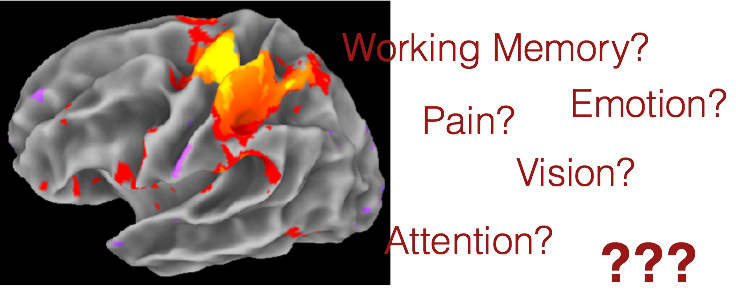
\includegraphics[height=4cm]{revinf.png}
\end{center}
\caption{The reverse inference problem}
\label{fig:revinf}
\end{figure}

\section{Related Work}
Forward and reverse inference problems have been addressed by several contemporary works~\cite{schwartz2013mapping, PMSKBY12, sanmi2013multi, yarkoni2011large}. Previous approaches have generally tackled the Reverse Inference problem by manually analyzing fMRI scans of subjects, collected from the laboratory. There are several limitations of such an approach - for instance, involving human subjects for fMRI scans is labor and cost intensive and the number of data samples that can be gained from such efforts is also very less. Moreover all the meta-analyses based on such data is carried on a very small-scale at individual research labs, and fails to take advantage of the vast knowledge embodied in the entire research community. We first present a detailed discussion of tje neurosynth approach before discussing other works.%In this report we will focus on neurosynth since it is most relevant to our approach. For a general discuss of other related works we request the reader to kindly refer to our proposal.

NeuroSynth's (and therefore our) approach is unique - in that we tackle the Reverse Inference problem not by requiring actual fMRI scans, but rather by exploiting the relatively large repository of neuro-imaging publications using text-mining and machine learning techniques.  There are many motivations and benefits that lead to this. For one, while fMRI scans are very few, there has been a growing body of publications related to neuro-imaging, thus offering a much larger source of data. Further by using machine learning techniques the decoding is possible without any real training data (fMRI scans) and at the same time incorporates the knowledge base derived from several researcher. Also to the best of our knowledge, this is the first approach that is fully automated, thus making it possible to perform several meta-analyses on a much larger scale than could ever be possible by individual researchers.  In the next few paragraphs, we introduce the NeuroSynth framework and some of the techniques it utilizes.

\subsection{The NeuroSynth framework}
\label{sec:neurosynth_framework}
The figure~\ref{fig:3steps} gives a high-level view of  NeuroSynth. 

\begin{figure}[h]
\begin{center}
%\framebox[4.0in]{$\;$}
%\fbox{\rule[-.5cm]{0cm}{4cm} \rule[-.5cm]{4cm}{0cm}}
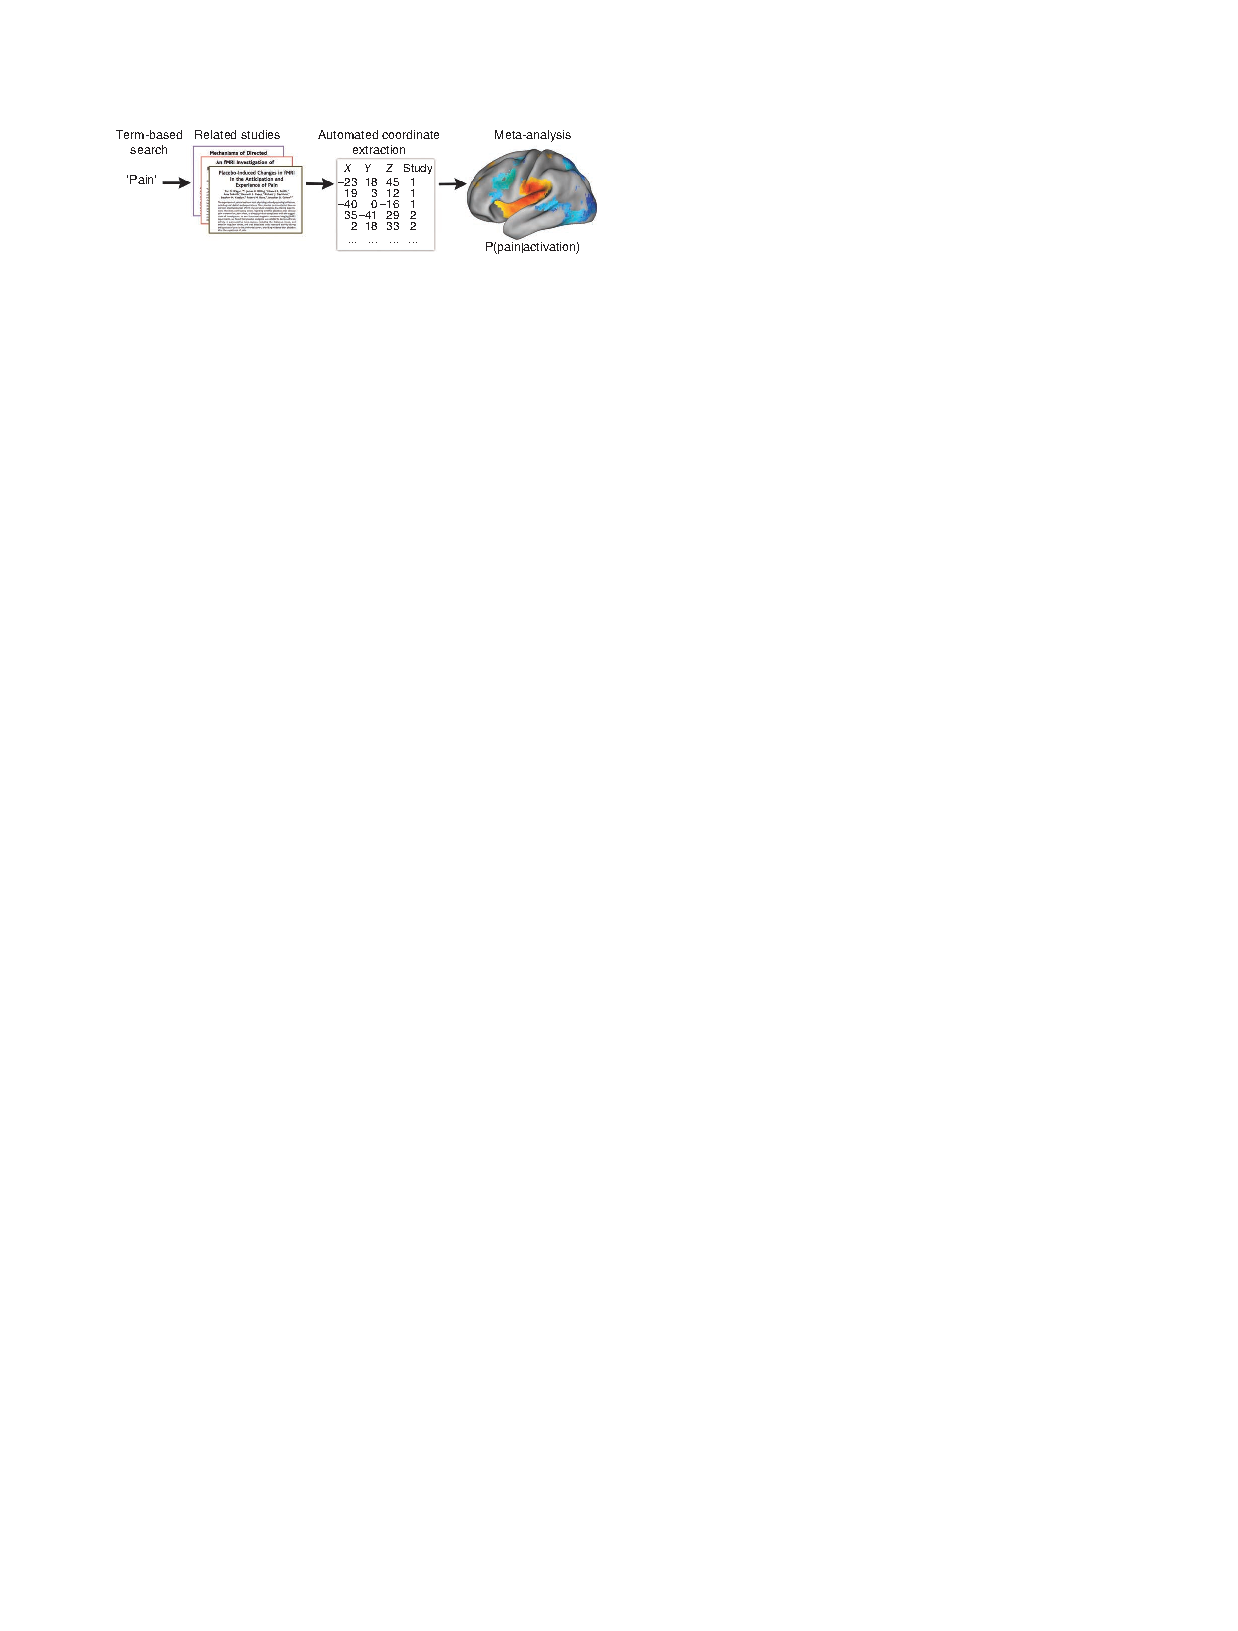
\includegraphics[height=4cm, width=14cm]{3steps.pdf}
\end{center}
\caption{The NeuroSynth framework~\cite{yarkoni2011large}}
\label{fig:3steps}
\end{figure}

A detailed description of NeuroSynth may be found in ~\cite{yarkoni2011large}. Here we give only a high-level view  - figure~\ref{fig:3steps}.  For reverse inference, NeuroSynth performs the following three steps:
\begin{description}
\item[Step 1:  Extract high frequency terms] First, a database of nearly $3000$-odd\footnote{The number has grown to over $8000$, since 2011 when ~\cite{yarkoni2011large} was published.} studies is scrapped to extract the most frequent terms and their frequency of occurence across these studies. Thus corresponding to each study we get a set of terms. These set of terms serve as labels for that study, during the classification.
\item[Step 2: Extract coordinates of activation foci and synthesize sparse image] Using simple template matching, all probable activation foci mentioned in a study are extracted. Once we have a list of these coordinates, corresponding to each study, they are used to synthesize extremely sparse brain images with the corresponding brain regions activated. After some preprocessing (which we describe in detail in section~\ref{sec:preprocess}) the vectorized image serves as the feature vector for that study.
\item[Step 3: Use classification to build a predictive model]  Use classification to train a model, given the labels and the feature vectors from steps (1) and (2). They use an extremely simple approach in which they apply a Naive Bayes classifier to make single-label predictions . They pick up $25$ of the most frequent terms arbitarily and train $25 \choose 2$ models (i.e one-vs-one) corresponding to every term pair and 10-fold cv to make the predictions.
\end{description}

There have been other approaches that have further built on NeuroSynth. For instance in ~\cite{sanmi2013multi}, the authors use label decomposition techniques in a one-vs-all setting to predict multiclass labels for the reverse inference problem. They use Support Vector Machines ($l_2$ regularized), logistic regression and ridge classifier for these tasks,  comparing the outcomes based on different criteria like precision, recall and Hamming loss, to show that the multiclass approach is effective for reverse inference. They also propose to use other multiclass approaches and regularization techniques and analyze their performance as future work. 

In another similar work~\cite{schwartz2013mapping} uses a Generalized Linear Model(GLM) for forward inference. For the reverse inference they use logistic regression with Ward clustering to counter the high dimensionality of the problem. 

Building up on these approaches,  in the following sections, we shall describe our own extensions and experiments toward building a better model for the reverse inference problem.

\subsection{Our Contribution}
 This work has three primary contributions
\begin{enumerate}
  \item We improve the single label prediction task by incorporating more sophisticated classifiers such as logistic regression, SVMs and ensembles.
  \item We experiment with several classifiers for the multilabel task. In particular we evaluate 6 different models of multilabel classifiers described in greater detail in Section~\ref{sec:methods}
  \item Finally we perform transfer learning using one of our better models from the multilabel task. We train our model on the synthesized neurosynth data and test it on a real fMRI database.
\end{enumerate}

\section{Methods}
\label{sec:methods}
 \paragraph{Notation}: We denote matrices by boldface capital letters $\mathbf{X}$ and vectors by bold-face lower case letters $\mathbf{x}$. The set of real valued $D$ dimensional vectors are denoted by $\mathbb{R}^D$. The set of (target) labels are denoted by the letter $\mathcal{L}$, and $|\mathcal{L}|$ denotes the cardinality of the set of labels.

Our input data consists of brain volume images. We denote by $\mathbf{x}_n$ the $n^{th}$ brain volume with voxels collected in a real valued $D$ dimensional vector. The total number of brain volumes is represented by $N$. Each brain volume is associated with a set of labels $\mathcal{L}_n = {l_1, \ldots, l_K}$ chosen from the full set of possible target labels $\mathcal{T} = \cup_{n=1,\ldots,N} \mathcal{L}_n$ with $|\mathcal{L}|=L$.

We approach the task of predicting brain functions as a classification task and address it using the following techniques:
 \subsection{Single Label Prediction}
  As a first step to measure the feasibility of the task we consider the task of predicting one of two labels for each brain volume. The single label prediction learns a mapping $f\ :\ \mathbf{x}_n \rightarrow \mathcal{L}_n$, such that $|\mathcal{L}_n|=1$ for all $n$, where $|\mathcal{T}| =| \cup \mathcal{L}_n| = 2$. This essentially learns a simple binary classifier for all pairs of labels. Each classifier is trained and tested on an appropriate subset of the data where the labels for the brain volume are unique. We experimented with the following binary classifiers:
  \begin{description}
  \item[Naive-Bayes] We built pairwise naive-bayes classifiers as a baseline to replicate the results presented in~\cite{yarkoni2011large}.
  \item[Logistic Regression] An $l_1$ regularized logistic regression was our next model of choice for a more powerful classifier.
  \item[Linear SVM] We use a linear SVM which scales well with the size of our features. The hyperparameter C is optimized by a grid search in the space $C = \{1, 10, 100, 1000\}$.
  \item[Ensemble] We finally build an ensemble of the above three classifiers and consider the label that is the majority in the output of the above three classifiers.
  \end{description}
\begin{figure}[ht]
\vspace{-0.5cm}
\centering
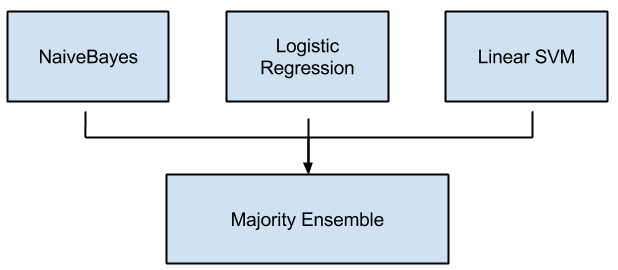
\includegraphics[scale=0.5]{./figs/single_pairwise.png}
\caption{We use naive-bayes, logistic regression, SVMs and a majority ensemble for pairwise binary classification of the labels.}
\end{figure}

 \subsection{Multi-Label Prediction} \label{subsec:method_multi}
Our next approach is to perform multilabel classification to predict multiple functions for a given brain volume. This learns a mapping $f\ :\ \mathbf{x}_n \rightarrow \mathcal{L}_n$, over the full set of labels (where $|\mathcal{L}_n| \geq 1$)  and $|\mathcal{T}| =| \cup \mathcal{L}_n|$. \cite{zhang2013review} suggests several methods to perform multilabel classification which include label projection, label ranking and label decomposition. We prefer the label decomposition method for it's ease of interpretation. In particular we choose the \textit{One-vs-All} decomposition approach. This method learns multiple binary classifiers ($|\mathcal{T}|$ to be precise), one for each label to predict the presence/absence of that label. Our experiments used the following binary classifiers for the multi-label prediction task:
  \begin{description}
  \item[Naive-Bayes] We built pairwise naive-bayes classifiers as a baseline to replicate the results presented in~\cite{yarkoni2011large}.
  \item[Logistic Regression] We build two models here. The first with $l_1$ or \textit{lasso} regularization and the other with $l_2$  or \textit{ridge} regularization. 
  \item[Linear SVM] In a manner similar to our single label prediction, we use a linear SVM by setting the hyperparameter C via a grid search in the space $C = \{1, 10, 100, 1000\}$.
  \item[Ward Clustering] Since the number of features in our data is extremely large, we do a dimensionality reduction of the features by first performing ward clustering [citation] and then mapping the points to different clusters. The number of clusters is 5000. We then apply a logistic regression classifier with $l_1$ regularization on the reduced data.
  \item[Unique train] Since our data is quite sparse and there's a high possibility of noise in data with multiple labels, we build what we call a unique train model based on logistic regression. In the unique train model, we identify all brain volumes with a single unique label, and train a classifier for each label using only this data. During test, we use the One-vs-All approach to test on multilabel brain volumes.
  \item[All ones] Another baseline we consider is the all ones baseline, which predicts ones for all labels on all input data points. Such a manipulation will give result in $100\%$ recall for the multilabel task, but very low precision values.
  \end{description}
In addition to the above, we did experiment with PCA and $k$-nearest neighbours for $k \in \{2,3,4\}$ but the models were not trained similarly or performed extremely poorly and hence we do not report results for these.
\begin{figure}[ht]
\vspace{-0.5cm}
\centering
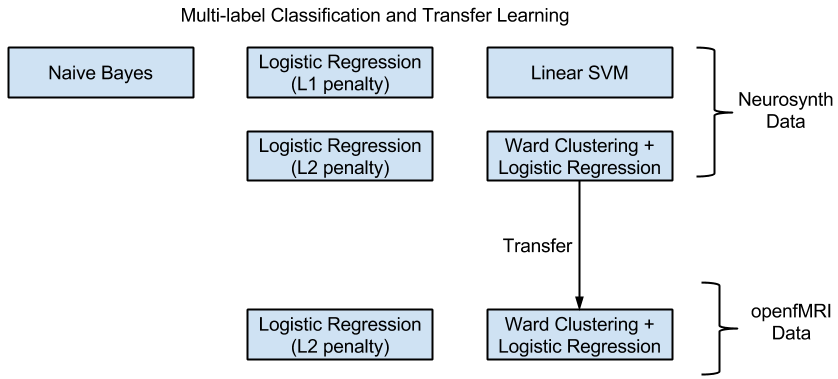
\includegraphics[scale=0.5]{./figs/multilabel_transfer.png}
\caption{We experiment several classifiers for the multilabel task. We pick our best performing models, namely logistic regression with $l_2$ penalty and the ward clustering based models and evaluate their performance on the openfMRI data. }
\end{figure}

 \subsection{Transfer Learning}
 As mentioned in Section~\ref{sec:neurosynth_framework}, one of the main purposes of this particular synthesis method for predicting brain functions is to be able to transfer the models from the synthesis domain to the real openfMRI domain. Based on the mapping functions that we learned in Section~\ref{subsec:method_multi} we want to apply the same function or a small modification of the function to new studies. That is, apply the mapping $f\ :\ \mathbf{x}_n \rightarrow \mathcal{L}_n$, to $\mathbf{x}'_n$ where ($\mathbf{x}'_n \notin \mathbf{X}$). In fact, our features $\mathbf{x}'_n$ are different both in dimension and constitution (the elements are continuous real valued data unlike the binary synthesis data). More details about the pre-processing is mentioned in Section~\ref{sec:preprocess}. In addition, we are interested in a predicting a different set of labels or functions, as constrained by the availability of data in the new domain. In effect, the transfer learning is attempting to learn $f'\ :\ \mathbf{x}'_n \rightarrow \mathcal{L}_n$. We experiment with the following methods here:
  \begin{description}
  \item[Ward Clustering] We reuse the ward clustering model that we learn previously by first performing ward clustering [citation] on the data in the synthesized domain to cluster and map the points to different clusters. We then train an $l_2$ regularized logistic regression \textit{One-vs-All} classifier on the data. Next we reapply the same clustering transformation to the openfMRI data and use the logistic classifier to predict the labels. The number of clusters is 5000.
  \item[Logistic Regression] For the sake of comparison we train an $l_2$ regularized logistic regression model directly on the openfMRI data.
  \end{description}
In this work we report the results for only the above two models. 

\section{Data}\label{sec:data}
Similar to ~\cite{yarkoni2011large}, we primarily use the repository available with NeuroSynth for our project. This has $8067$ studies that are scrapped from online resources, spanning $15$ journals. For our transfer-learning approach, we would like to use real fMRI scans, and adapt our models tuned with the synthesized data on this real data. We use data from 2 sources. We use the open source openfMRI~\footnote{\protect \url{https://openfmri.org}} project ~\cite{poldrack2013toward} to gain the training data. This has individual subject level images for $26$ contrasts, resulting in a total of $479$ data samples. Since it is always more advisable to work with group level statistics, we also consider the NeuroVault\footnote{\protect \url{http://neurovault.org}} data that has 17 studies, but with group level images. Ideally we would have liked to use this data entirely but the major issues is that it is too less to be meaningful on its own. 
\subsection{Pre-processing}
\label{sec:preprocess}
Here we describe mainly the preprocessing pipe for the NeuroSynth data. The code repository for NeuroSynth already has the labels and coordinates that are extracted from the $8067$ studies. Beginning with this, we used various open source toolkits like NumPy tand existing utiliities in NeuroSynth to synthesize images corresponding to the the activated coordinates. 

\begin{description}
\item[Step 1: ] First for each $(x, y, z)$ coordinate extracted from a study, we transformed it to the MNI space - which is the standard space used for neuro-imaging. 
\item[Step 2: ] Second, since the coordinates were extracted using simple template matching, there would likely be some spurious numbers that were mistaken as coordinates. It is also possible that the study mentioned coordinates for some different region other than the brain. To deal with such anomalies, we then applied a 2mm MNI mask on the coordinates, to validate that they indeed lay in the brain space and discarded the invalid ones. The 3D mask has the shape $(91 \times 109 \times 91)$ 
\item[Step 3: ] Since each study mentions only a very few coordinates from the entre brain space, the resulting image we would get would be extremely sparse. Based on connectivity and correlation amongst the brain regions, given an activated focus, it is highly likely that the voxels in its neighbourhood would be actvated as well. Using this fact we considered all voxels in a $6$ mm radius around the activated foci to also be activated and thus get a more dense and smoother image.
\item[Step 4: ] Once we get this synthesized image in $3$D MNI space, we reshape it to a $1$D vector, further removing all zero-columns, to end up with a $1 \times 228453$ feature vector.  
\end{description}

Since the data is extracted based on simple text processing, there will likely be irrelevant data that is also included. To deal with this we apply some further steps, in which we only consider terms that have a normalized frequency count $ > 0.001$. Further we only consider those studies to be valid, that have atleast 500 activated voxels in the final feature vector. Further for single-label classification we only consider studies, that have a unique label with normalized frequency  $ > 0.001$. Studies that have multiple labels at a frequency $ > 0.001$ cannot e clearly assigned a single correct label, and we therefore do not consider them for the single-label classification problem.

For the sake of comparibility, we use the same $22$ terms as labels for our experiments as~\cite{yarkoni2011large}\footnote{The paper actually considers $25$ terms however, $3$ of these were absent in the version of the data we worked with} . After we perform the filtering steps we mentioned above, we end up with a total of $2464$ studies out of the original $8067$ studies, for the single label classification task.

For the multi-label classification, we perform the same filtering and pre-processing as mentioned above, the only difference being that this time we allow multiple labels per study, instead of removing the studies with conflicting labels. Thus we end up with a total of $5463$ studies from the original $8067$ studies. Similar to ~\cite{sanmi2013multi} we plot a histogram that shows the distribution of terms across studies (fig~\ref{fig:histo_old}). 

\begin{figure}[h]
\begin{center}
%\framebox[4.0in]{$\;$}
%\fbox{\rule[-.5cm]{0cm}{4cm} \rule[-.5cm]{4cm}{0cm}}
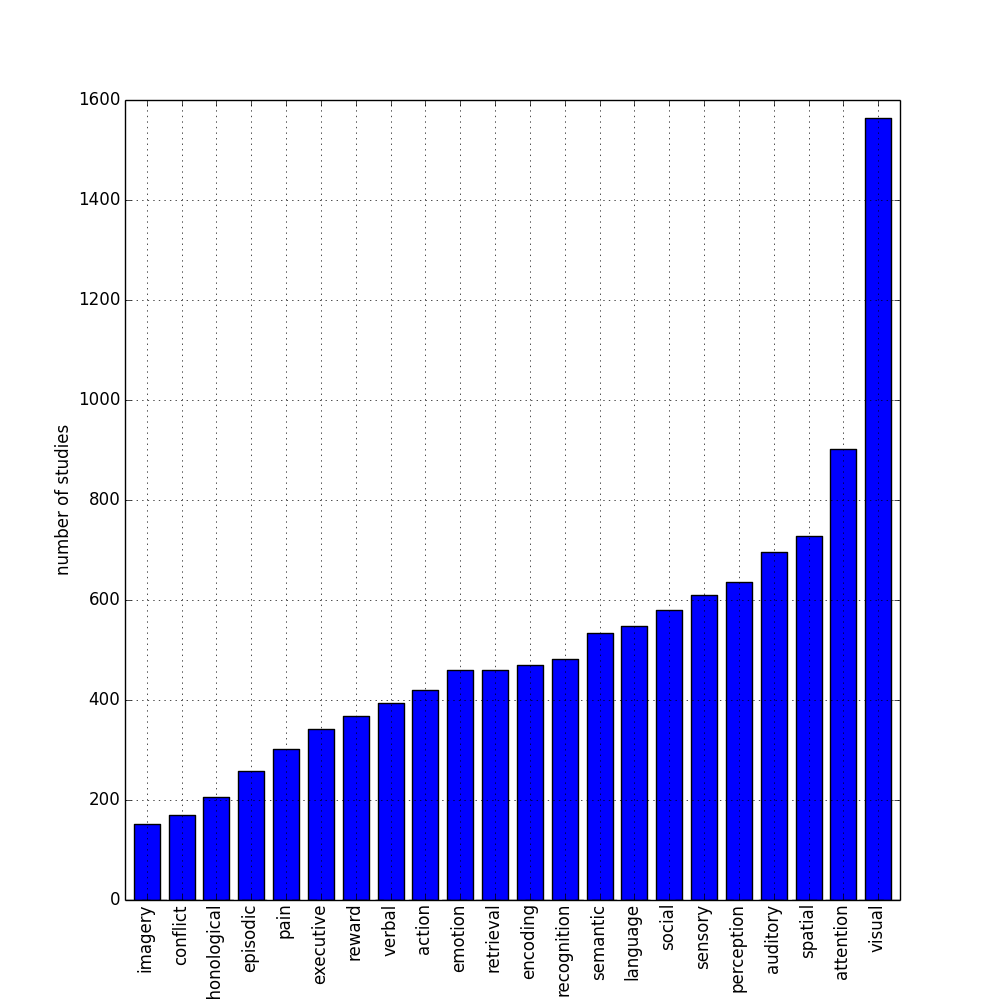
\includegraphics[height=10cm, width=10cm]{histo_old.png}
\end{center}
\caption{\textbf{Distribution of terms across studies:} The x-axis denotes each term and the y-axis denotes the number of studies (in the NeuroSynth database) in which the terms appears.}
\label{fig:histo_old}
\end{figure}

\subsection{OpenfMRI and Neurovault text extraction}

For the purposes of transfer learning we use the openfMRI and NeuroVault repositories as a source of real fMRI data. The openfMRI data is also in a similar format to the NeuroSynth data.  Thus there is a study associated with an fMRI image and these have already been text-processed previously, to give a frequency count for some $19$ terms of interest.  One issue is that the labels in NeuroSynth do not overlap the labels that were extracted for openfMRI. Thus we pick out terms tha would be similar to the openfMRI terms from the NeuroSynth database. Now using these new $19$ terms, we perform a simialr preprocessing as in the multi-label case to filter out studies that would be reliable for these new terms of interest. We end up with $4066$ such studies from the NeuroSynth database. Again a distribution of different terms across the studies is presented in fig~\ref{fig:histo_new}.

\begin{figure}[h]
\begin{center}
%\framebox[4.0in]{$\;$}
%\fbox{\rule[-.5cm]{0cm}{4cm} \rule[-.5cm]{4cm}{0cm}}
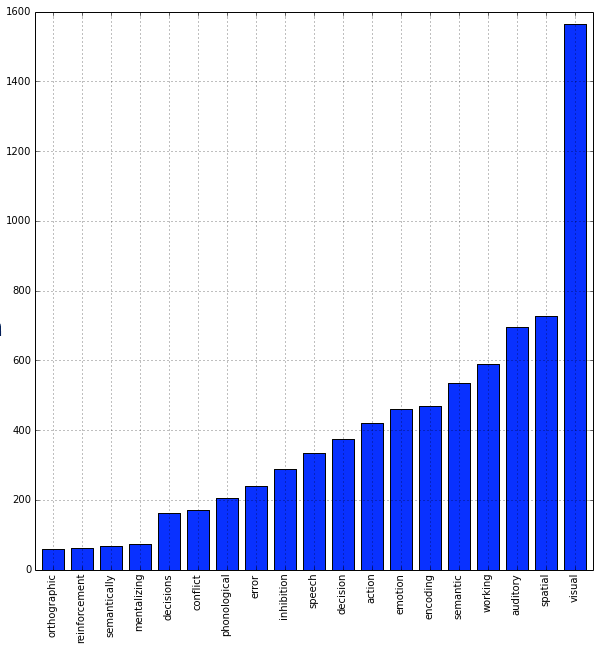
\includegraphics[height=10cm, width=10cm]{histo_new.png}
\end{center}
\caption{\textbf{Distribution of terms across studies:} The x-axis denotes eac term and the y-axis denotes the number of studies in which the term appears.}
\label{fig:histo_new}
\end{figure}

For NeuroVault, the data was not available in a format similar to the openfMRI and NeuroSynth. In this case, we had a total of 17 images, that corresponded to 12 studies. Rather than having the actual labels for these studies, the API provided us with links to online publications corresponding to the study. These were in the \texttt{pdf} format, though in some cases, mutliple formats were also available. We used an approach similar to that already adopted by NeuroSynth, to derive labels for the images. First we converted the \texttt{pdf} formats to plain text using an available python tool~\footnote{http://www.unixuser.org/~euske/python/pdfminer/}. Next we considered a dictionary of terms which we were using for the Neurosynth data and counted how frequently these terms appeared in each study. The final frequency we stored for these terms was normalized by dividing it by the total word count of the document. Thus we ended up with a label representation for each study that was analogous to what was being used in NeuroSynth.

\section{Experimental Results}

Our experiments for single and multilabel prediction tasks were performed on data available in the NeuroSynth~\footnote{\protect \url{www.neurosynth.org}} tool. After preprocessing and filtering our inpput feature matrix  $\mathbf{X}$ is of dimension $5463 \times 228,453$, the target label matrix $\mathbf{Y}$ is of dimension $5463 \times 22$. The transfer learning component is tested on data from the openfMRI~\footnote{\protect \url{https://openfmri.org}} project with feature dimensions $\mathbf{X}'$ ($479 \times 174,264$) and target label matrix $\mathbf{Y}'$ of dimensions $479 \times 19$. As mentioned in Section~\ref{sec:data} we the labels for the transfer learning is a different set of 19 terms. The neurosynth data features for the transfer learning had dimensions $4066 \times 174,264$.

Data samples size (4000). We use 10 fold cross validation to evaluate all our models unless otherwise indicated. We evaluate the performance of our models on the metrics such as \textit{accuracy, precision, recall, hamming loss, F1 score} which are frequently applied to this task.
\begin{align*}
 \text{Accuracy} &= \frac{1}{N} \displaystyle\sum_{n=1}^{N} \frac{|\mathcal{L}_n \cap \mathcal{Z}_n|}{|\mathcal{L}_n \cup \mathcal{Z}_n|} 
\end{align*}

 \subsection{Single Label Prediction}
 We present the accuracies of the pairwise single label predictions using all our approaches in the heat maps in Figures~\ref{fig:singlelab1} and \ref{fig:singlelab2}
\begin{figure}[!hbt]
\vspace{-0.5cm}
\centering
\subfloat[Naive Bayes]{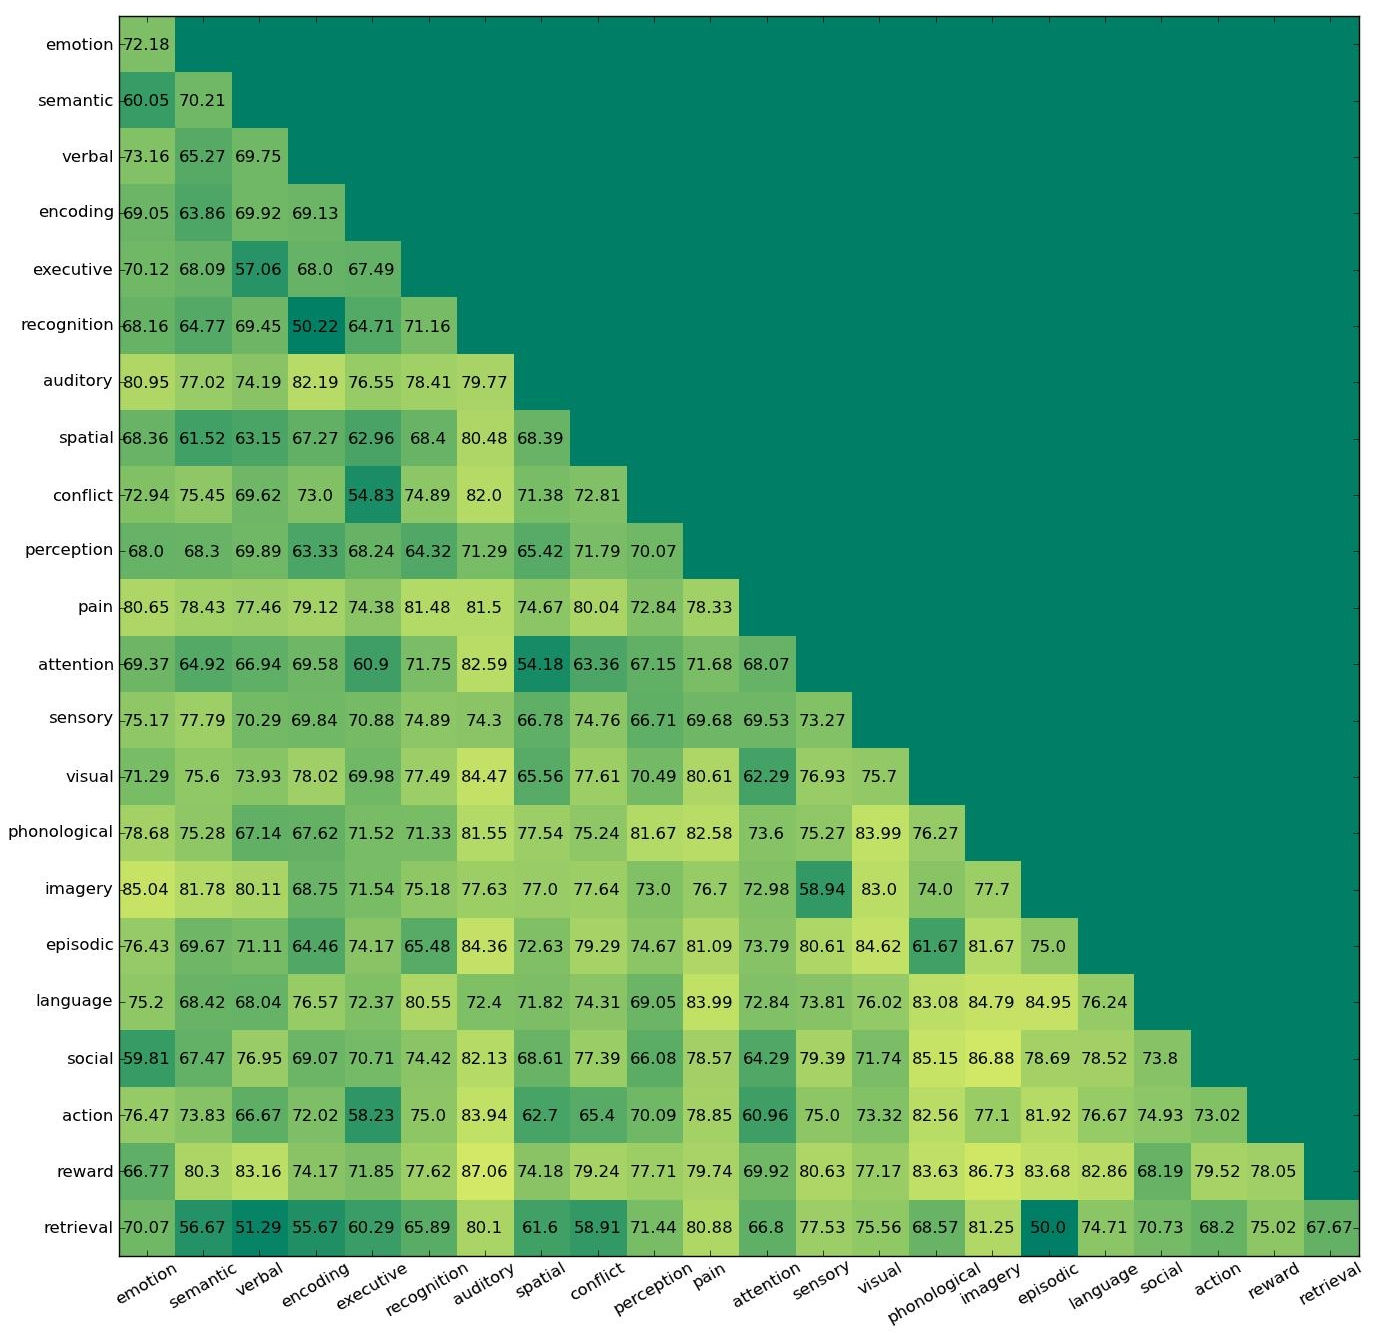
\includegraphics[width=10cm]{./figs/nb_confmat.jpg}} \\
\subfloat[Logistic Regression]{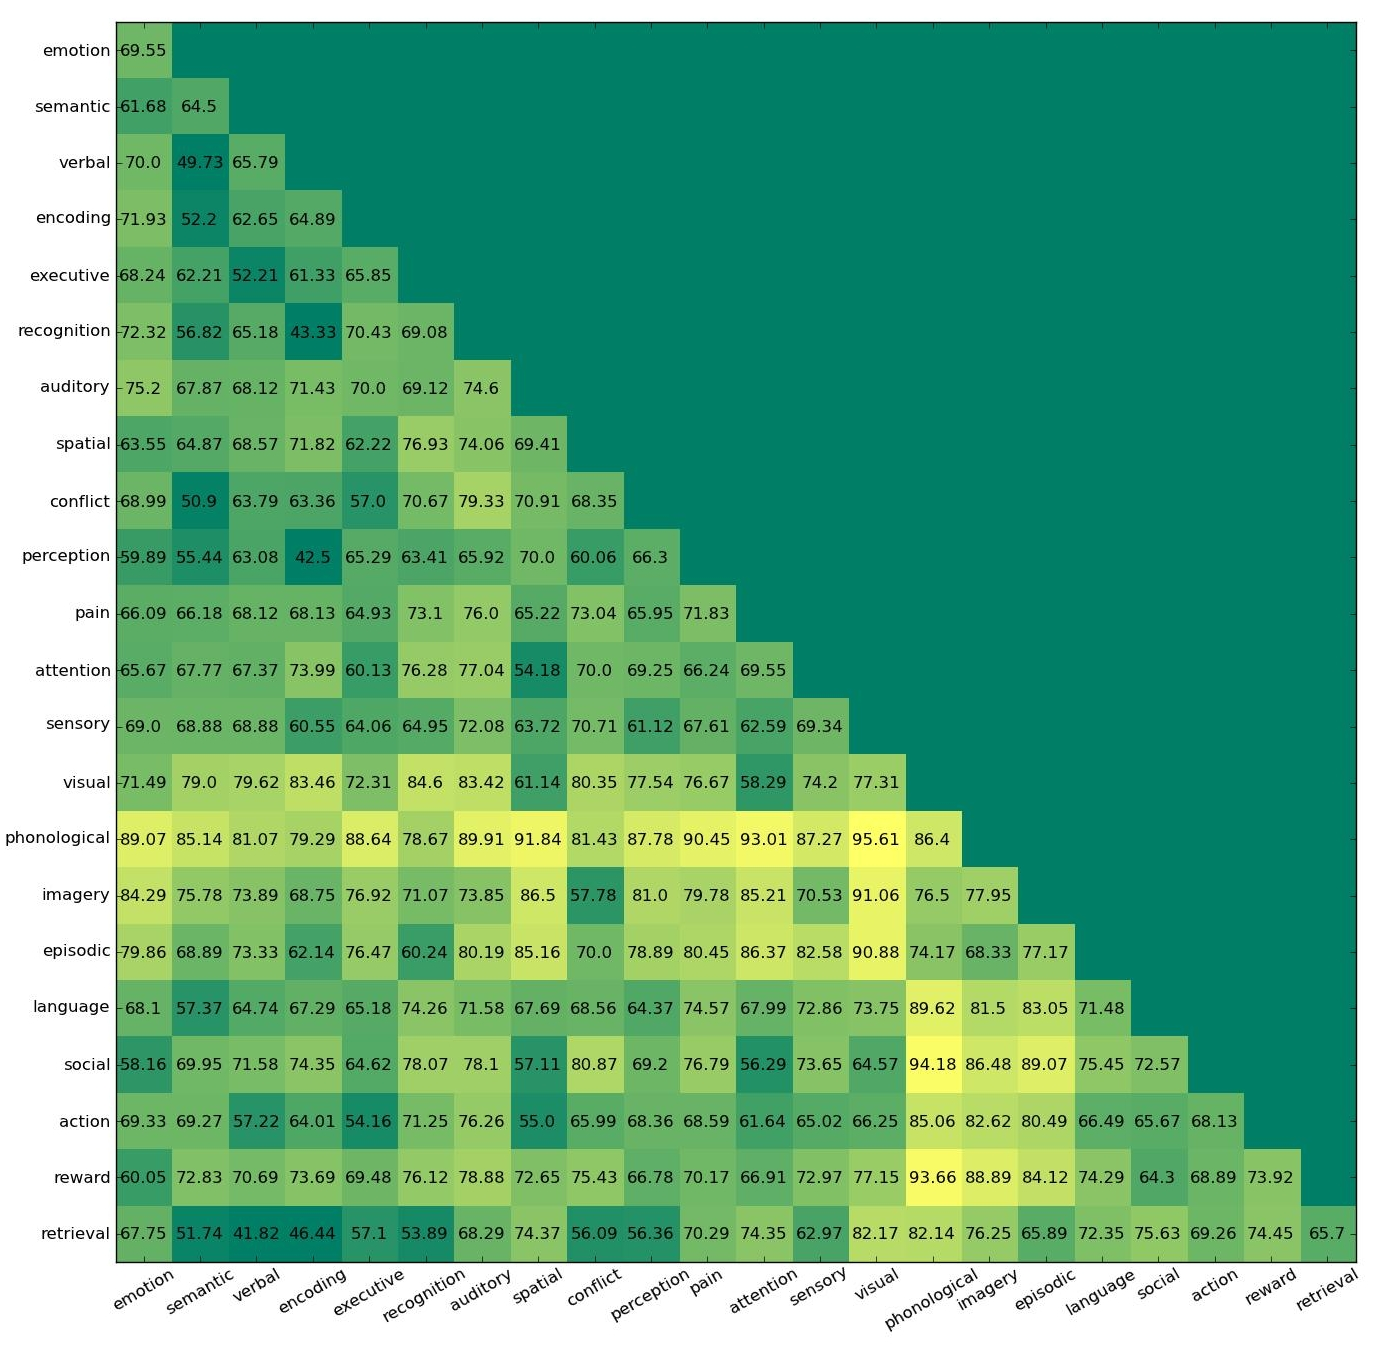
\includegraphics[width=10cm]{./figs/log_confmat.jpg}}
\caption{Pairwise binary classification accuracy for single label prediction}
\label{fig:singlelab1}
\end{figure}
\begin{figure}[!hbt]
\vspace{-0.5cm}
\centering
\subfloat[Linear SVM]{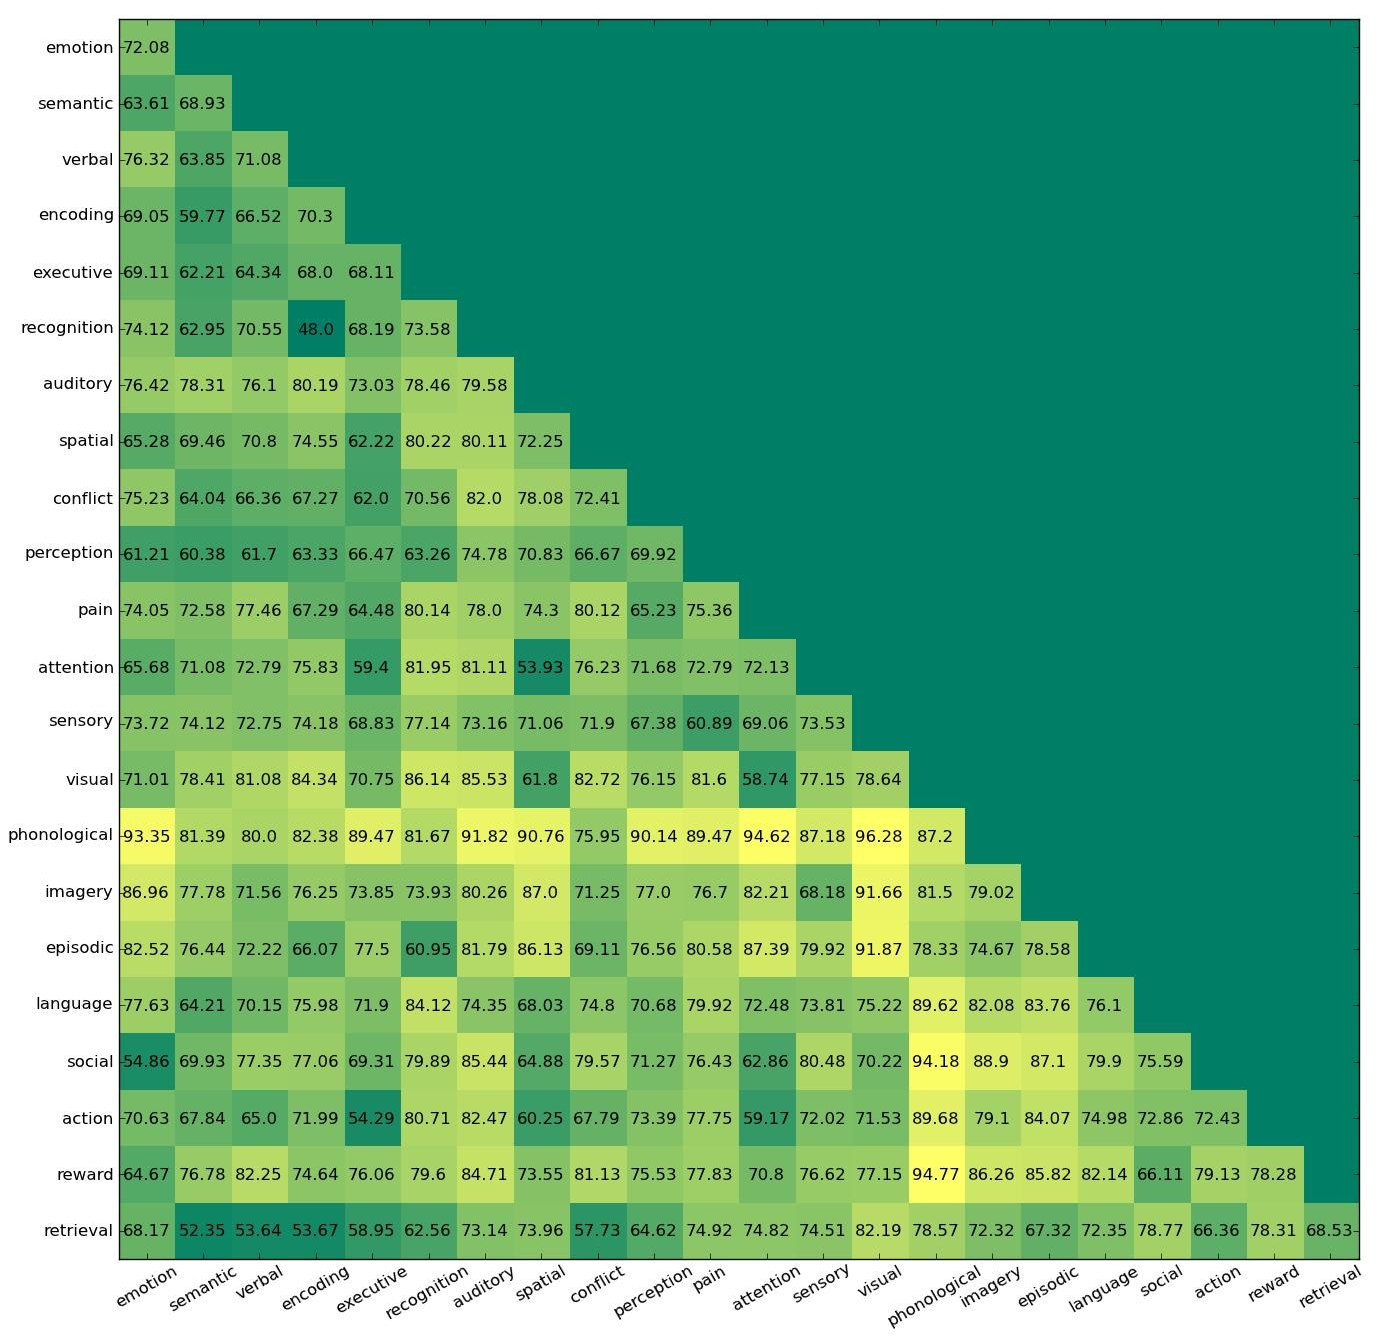
\includegraphics[width=10cm]{./figs/svm_confmat.jpg}} \\
\subfloat[Ensemble of naive bayes, logistic regression and SVM]{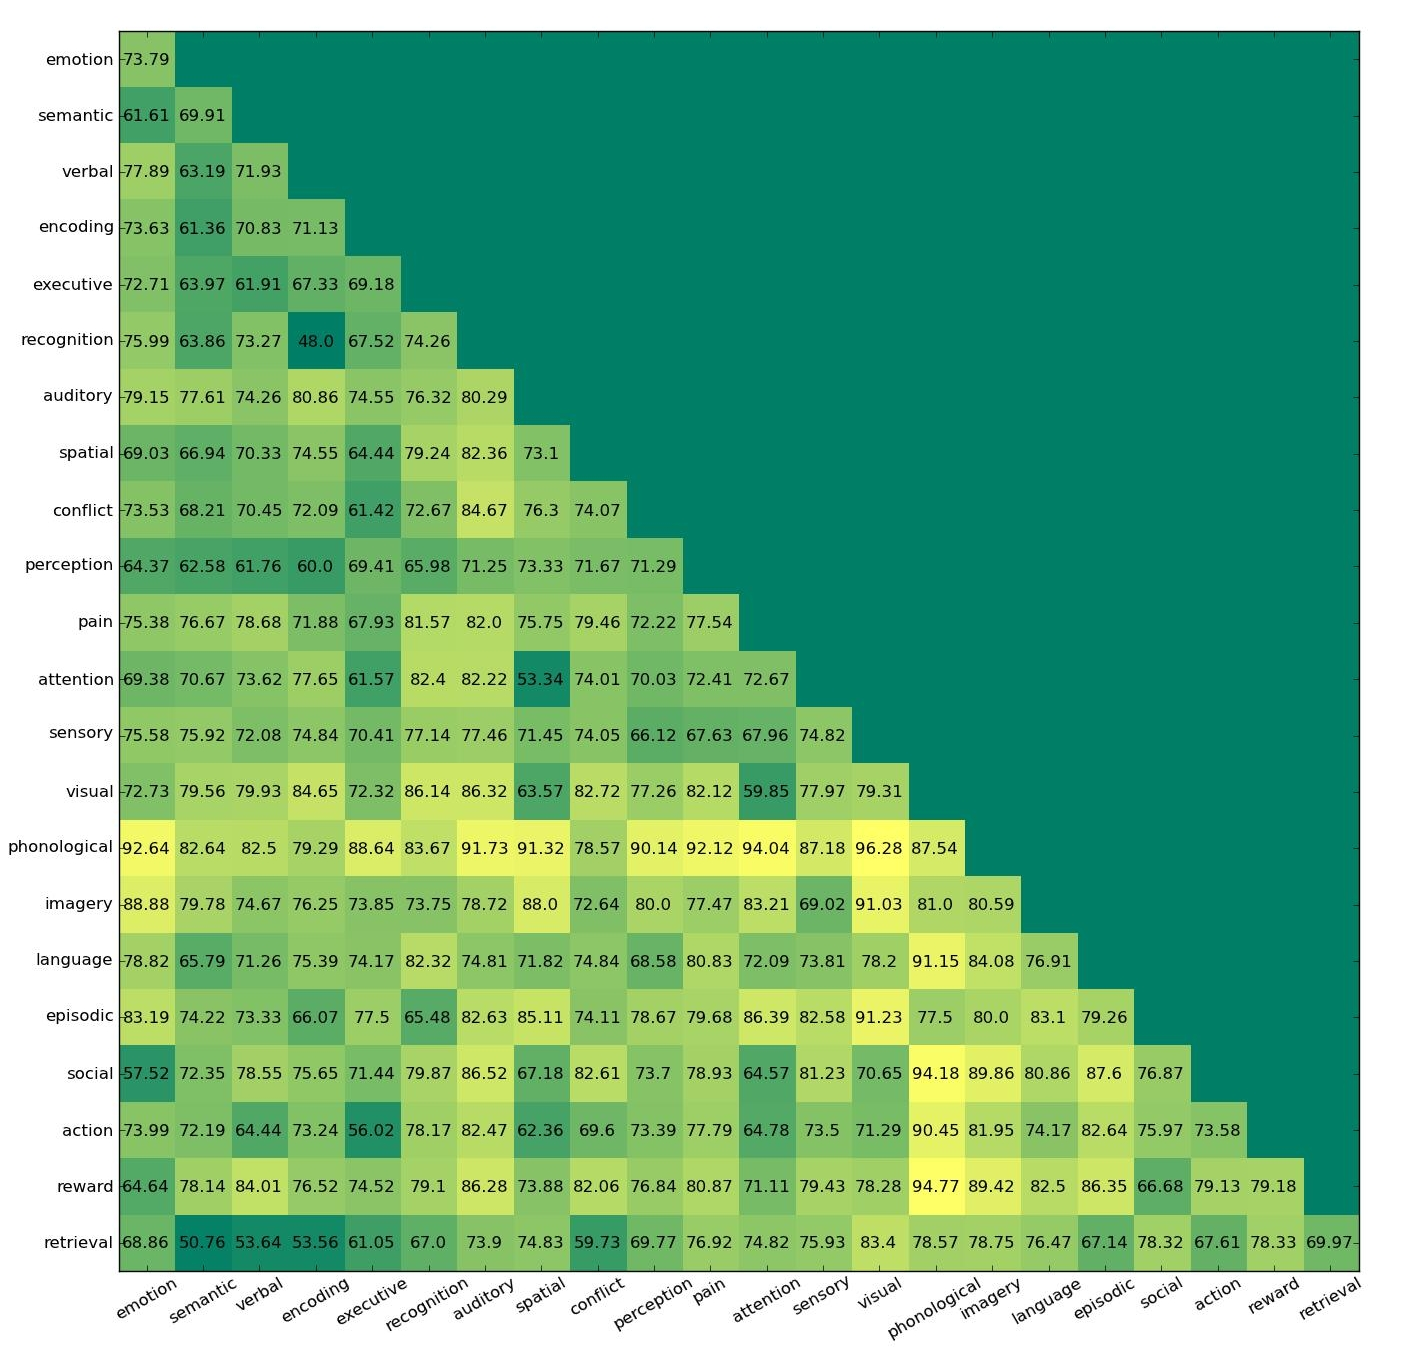
\includegraphics[width=10cm]{./figs/ensemble_confmat.jpg}}
\caption{Pairwise binary classification accuracy for single label prediction}
\label{fig:singlelab2}
\end{figure}

\paragraph{Discussion} Our Naive Bayes model performs comparably to the results reported in ~\cite{yarkoni2011large}. The results are quite good given the assumptions and simplicity underlying the model, as well as the large dimensions of our data.
Terms like phonological, pain and visual have a very high accuracy. We note that adding sophisticated models does improve the accuracy significantly for a good number of pairs. For logistic regression, we see that the model beats Naive Bayes for many pairs (Figure\ref{fig:singlelab1} bottom half is brighter). For instance
terms like phonological which had a high accuracy in Naive Bayes, show an even higher accuracy here, improving by $5-8\%$. But in a few cases, the accuracy also dips by a factor of $2-3\%$.
The Linear SVM shows a trend similar to the logistic regression, improving the accuracy for the high accuracy terms from Naive Bayes as well as logistic regression. But the SVM does have a slight edge over the logistic regression model. As was expected, the ensemble model of the three is the clear winner, although it only marginally beats the SVM.

 \subsection{Multi-Label Prediction}
In addition to reporting the accuracy, we report precision, recall, F1 score and hamming loss. And one correct
\begin{align*}
 \text{Precision} &= {1}{N} \sum_{n=1}^{N} \frac {|\mathcal{L}_n \cap \mathcal{Z}_n|}{\mathcal{Z}_n}& \text{Recall}&= \frac{1}{N} \sum_{n=1}^{N} \frac {|\mathcal{L}_n \cap \mathcal{Z}_n|}{\mathcal{L}_n}\\
 \text{F1 score} &=\frac{1}{N} \sum_{n=1}^{N} \frac{2.0 * \text{Precision}_n * \text{Recall}_n}{\text{Precision}_n +\text{Recall}_n} & \text{Hamming loss}&=\frac{1}{N}\sum_{n=1}^{N}\frac{1}{L} |\mathcal{L}_n \ominus \mathcal{Z}_n | \\
 \text{Top correct} &=\frac{1}{N} \displaystyle\sum_{n=1}^{N} \mathbb{I}(\mathcal{Z}_{n,max} \in \mathcal{L}_n)& & \\
\end{align*}
$\mathbb{I}$ denotes the indicator function and $\mathcal{Z}_{n,max}$ denotes the label predicted with highest probability for the brain volume $n$. The top correct value is the fraction of the data points on which the model's best predicted label (with maximum probability) was present in the true label set.

This table reports the results of the multilabel classification for the entire label set. Note here that there are $2^{22}$ possible label sets and accuracy is a fairly hard metric to achieve
\begin{table}[h]
\begin{center}
\begin{tabular}{|c|c|c|c|c|c|c|}
\hline
 Model       & Accuracy & Precision & Recall    & F1 score  & Hamming loss & Top correct\\ \hline
 Naive Bayes & 1.3      & \bf{22.36}& \bf{46.04}& \bf{26.63}& 0.207     & 23.7      \\ \hline
 Logistic L1 & 3.2      & 18.92     & 14.16     & 14.53     & 0.111     & 27.9      \\ \hline
 Logistic L2 & \bf{4.1} & 19.58     & 14.73     & 15.22     & 0.108     & \bf{30.0} \\ \hline
 Linear SVM  & 3.7      & 20.34     & 16.40     & 16.24     & 0.115     & 22.5      \\ \hline
 Ward Cluster& 3.4      & 17.53     & 12.99     & 13.43     & \bf{0.107}& 29.8      \\ \hline \hline
 Unique Train$^*$& 0.8      & \bf{33.98}& 22.09     & 24.83     & 0.162     & \bf{36.0} \\ \hline
 All Ones$^*$    & 0.0      & 9.78      & \bf{100.0}& 17.40     & 0.902     & 5.38      \\ \hline
\end{tabular}
\caption{Multilabel classification full tuple results. All values are reported in percentage ($\%$) except hamming loss. Again, excepting for hamming loss where lower loss is better, for all other metrics higher values are better. $^*$Unique Train and All Ones do not use cross validation.}
\end{center}
\end{table}
\paragraph{Discussion}
The multilabel task is a much harder task. It appears that our model does quite poorly on getting entire set of labels correct. This was to be expected given the huge dimensional and sparse data, but more importantly the set of potential labels is $2^22$ which is $4194304$. Considering such a huge set possible labels, an accuracy of $4.1\%$ does seem significant.
We note that the best performing models for the overall accuracy are the SVM ($3.7\%$) and  $l-2$ regularized logistic regression ($4.1\%$). Almost all of our models show a healthy hamming loss. However, the simplest naive-bayes model appears to be the best performing in terms of precision, recall and F1 score.  The model using Ward Clustering shows the best performance for the Hamming Loss metric. Also the Unique train model does the best on the Top correct metric, picking out atleast one correct label on $36\%$ of the cases.

Our intuition for including the Top correct metric was to make a judgement on how well our individual classifiers are performing. It appears that on average for $27\%-30\%$ of the brain volumes the models is able to predict atleast one relevant label which seems very promising.


 \subsection{Transfer Learning}
This table reports the results of the transfer learning for the entire label set. We get 0 accuracy for the full label set and hence do not report the value in the table below.
\begin{table}[h]
\begin{center}
\begin{tabular}{|c|c|c|c|c|c|c|}
\hline
 Model           & Precision & Recall    & F1 score  & Hamming loss & Top correct\\ \hline
 Logistic L2     & \bf{24.05}& 28.04     & \bf{21.24}& \bf{0.280}   & \bf{31.57} \\ \hline
 Ward Cluster$^*$& 13.63     & \bf{35.35}& 16.92     & 0.416        & 12.09      \\ \hline
\end{tabular}
\caption{Multilabel classification full tuple results. All values are reported in percentage ($\%$) except hamming loss. Again, excepting for hamming loss where lower loss is better, for all other metrics higher values are better. $^*$ Note here that the logistic regression model is some sort of an upper baseline since it is being trained on the openfMRI data whereas clustering is trained on neurosynth and the model is directly applied to the openfMRI data. Clustering does not employ cross validation since the training and test set are from different datasets.}
\end{center}
\end{table}

\paragraph{Discussion}
Similar to the multi-label case, the results that we obtain are not sufficiently encouraging. But compared to the topline approach ,the $l_2$ regularized logistic regression which is trained and tested on the same data, the transfer learning shows some hope. We would like to reiterate here that the input data dimensions and the target labels for the openfMRI are quite different from the models on which the multilabel classification experiments were performed. We are looking for better methods to tune the transfer.

\subsection{We also tried ...}
As mentioned previously, we also considered the nearest neighbour technique for both multilabel and transfer learning approaches. But due to extreme sparsity of data the model performed very poorly (with neighbours $k=2,3,4$) and hence we have not discussed that here. We also experimented with PCA for dimensionality reduction. However, we had issues specific to running it on the tacc cluster (with regard to .mkl libraries for C). So, we were unable to test our model on the large dataset. We should probably consider other dimensionality reduction techniques before doing the classification task.

With regard to transfer learning, we would like to mention that we also considered and built a model (based off NeuroSynth) that uses pearson correlation distance to measure correlation between a new image and averaged voxel values for each label. i.e. We build one vector for each label by averaging the voxel values that are activated by all images marked with the label. We then use pearson correlation to compare a new image vector with the averaged vector for each of the labels. However, this was not amenable to the transfer approach because of the different dimensions of the new openfMRI data. 

\section{Conclusion}
In this project we explored several classification algorithms for the task of predicting mental functions from brain activations. We approached the task as identifying single labels for each brain volume, then as a multilabel classification problem to classify synthesized brain volumes. The final main objective was to perform transfer learning by applying our models to real fMRI data. From our experiments there was no one single model that worked well on all tasks (and all metrics). SVMs and logistic regression classifiers (with $l_2$ penalty) worked very well on label classification tasks giving very high accuracy. However, the simple Naive Bayes model was not too far behind and performed well on precision, recall and F1 score, particularly on the multilabel task.

Overall, the results we have seem rather poor. But we are not clearly able to identify the reasons for this. One strong future direction to proceed in would be to do dimensionality reduction and redo the experiments and that might give us better results. However, the only consolation that we have is that the task is pretty hard and all of our models definitely beat simple baselines by a large margin.

\subsubsection*{Acknowledgments}
We are very thankful to Tal Yarkoni and Dr Russ Poldrack, from the Image Research Centre, University of Texas at Austin, for their
helpful suggestions and tips. We are especially grateful to  Oluwasanmi (Sanmi) Koyejo, who patiently guided us through this entire project.
We cannot fail to mention the excellent TACC resources, without which it would have been impossible to run experiments at this scale.
Finally we would like to thank Prof Ghosh for teaching us many practical nuances in the course that helped immensely during the project.

\bibliographystyle{plain}
\nocite{*}
\bibliography{brain_function_prediction.bib}

\section{Appendix}

We report statistics per label for each of our multilabel experiments:
\begin{table}[h]
\begin{center}
\begin{tabular}{ll}
\begin{tabular}{|c|c|c|c|c|}
\hline
 \bf{Label}  & \bf{Accuracy} & \bf{Precision} & \bf{Recall}    & \bf{F1 score} \\ \hline
action	& 13.32	& 16.78	& 38.92	& 23.33	\\ \hline 
attention	& 16.84	& 23.75	& 36.75	& 28.73	\\ \hline 
auditory	& 29.47	& 38.07	& 57.13	& 45.20	\\ \hline 
conflict	& 4.51	& 5.81	& 17.46	& 8.53	\\ \hline 
emotion	& 14.68	& 17.26	& 50.87	& 25.52	\\ \hline 
encoding	& 11.64	& 15.42	& 31.85	& 20.70	\\ \hline 
episodic	& 10.38	& 12.14	& 42.52	& 18.69	\\ \hline 
executive	& 8.11	& 10.86	& 25.49	& 14.88	\\ \hline 
imagery	& 5.74	& 6.92	& 25.15	& 10.52	\\ \hline 
language	& 20.68	& 26.02	& 50.14	& 34.12	\\ \hline 
pain	& 19.37	& 21.52	& 69.06	& 32.41	\\ \hline 
perception	& 12.88	& 17.34	& 33.30	& 22.73	\\ \hline 
phonological	& 11.51	& 13.13	& 49.54	& 20.61	\\ \hline 
recognition	& 11.66	& 15.12	& 33.92	& 20.75	\\ \hline 
retrieval	& 14.13	& 17.70	& 41.00	& 24.51	\\ \hline 
reward	& 16.18	& 18.85	& 55.01	& 27.69	\\ \hline 
semantic	& 17.72	& 21.54	& 49.52	& 29.94	\\ \hline 
sensory	& 14.21	& 19.00	& 35.87	& 24.73	\\ \hline 
social	& 17.10	& 20.69	& 49.34	& 29.01	\\ \hline 
spatial	& 19.50	& 25.37	& 45.89	& 32.55	\\ \hline 
verbal	& 10.33	& 13.73	& 29.91	& 18.64	\\ \hline 
visual	& 34.78	& 47.08	& 57.20	& 51.55	\\ \hline 
\end{tabular}
&
\begin{tabular}{|c|c|c|c|}
\hline
 \bf{Accuracy} & \bf{Precision} & \bf{Recall}    & \bf{F1 score} \\ \hline
 3.92	& 14.86	& 5.09	& 7.37	\\ \hline 
 8.71	& 23.10	& 12.26	& 15.92	\\ \hline 
 24.05	& 52.10	& 30.70	& 38.39	\\ \hline 
 2.64	& 15.33	& 3.21	& 4.81	\\ \hline 
 8.16	& 25.92	& 10.60	& 14.78	\\ \hline 
 7.23	& 27.76	& 8.84	& 13.27	\\ \hline 
 6.91	& 23.62	& 9.17	& 12.48	\\ \hline 
 1.84	& 8.33	& 2.24	& 3.46	\\ \hline 
 1.22	& 10.00	& 1.30	& 2.30	\\ \hline 
 10.51	& 31.65	& 13.66	& 18.86	\\ \hline 
 13.01	& 40.69	& 16.07	& 22.55	\\ \hline 
 5.76	& 20.59	& 7.39	& 10.65	\\ \hline 
 7.77	& 25.56	& 10.22	& 13.80	\\ \hline 
 3.93	& 16.03	& 4.92	& 7.42	\\ \hline 
 7.56	& 24.23	& 9.56	& 13.52	\\ \hline 
 17.69	& 40.78	& 23.43	& 29.36	\\ \hline 
 8.53	& 27.02	& 10.98	& 15.53	\\ \hline 
 3.07	& 10.34	& 4.07	& 5.77	\\ \hline 
 7.89	& 23.36	& 10.77	& 14.52	\\ \hline 
 8.15	& 26.85	& 10.67	& 14.92	\\ \hline 
 2.30	& 10.50	& 2.88	& 4.45	\\ \hline 
 22.05	& 41.07	& 32.12	& 35.98	\\ \hline 
\end{tabular}
\end{tabular}
\caption{Multilabel, per label accuracy naive bayes (left table) and logistic regression with $l_1$ penalty (right table)}
\end{center}
\end{table}

\begin{table}[h]
\begin{center}
\begin{tabular}{ll}
\begin{tabular}{|c|c|c|c|c|}
\hline
 \bf{Label}  & \bf{Accuracy} & \bf{Precision} & \bf{Recall}    & \bf{F1 score} \\ \hline
action	& 5.00	& 19.44	& 6.29	& 9.45	\\ \hline 
attention	& 7.27	& 20.33	& 10.24	& 13.49	\\ \hline 
auditory	& 25.44	& 52.52	& 32.56	& 40.03	\\ \hline 
conflict	& 0.00	& 0.00	& 0.00	& 0.00	\\ \hline 
emotion	& 7.23	& 28.24	& 9.06	& 13.46	\\ \hline 
encoding	& 4.45	& 21.41	& 5.47	& 8.48	\\ \hline 
episodic	& 6.17	& 29.83	& 7.19	& 11.29	\\ \hline 
executive	& 1.57	& 18.67	& 1.70	& 3.02	\\ \hline 
imagery	& 0.00	& 0.00	& 0.00	& 0.00	\\ \hline 
language	& 9.76	& 30.04	& 12.72	& 17.68	\\ \hline 
pain	& 11.99	& 49.25	& 14.34	& 20.89	\\ \hline 
perception	& 6.13	& 19.32	& 8.20	& 11.42	\\ \hline 
phonological	& 6.50	& 34.88	& 7.60	& 11.54	\\ \hline 
recognition	& 4.84	& 23.66	& 5.76	& 9.10	\\ \hline 
retrieval	& 7.02	& 28.40	& 8.44	& 12.89	\\ \hline 
reward	& 19.70	& 53.50	& 24.11	& 32.52	\\ \hline 
semantic	& 8.76	& 28.81	& 11.16	& 15.96	\\ \hline 
sensory	& 4.48	& 16.64	& 5.86	& 8.53	\\ \hline 
social	& 7.46	& 23.98	& 9.75	& 13.75	\\ \hline 
spatial	& 10.72	& 29.31	& 14.59	& 19.18	\\ \hline 
verbal	& 3.35	& 22.58	& 3.85	& 6.38	\\ \hline 
visual	& 23.92	& 42.96	& 35.03	& 38.51	\\ \hline 
\end{tabular}
&
\begin{tabular}{|c|c|c|c|}
\hline
 \bf{Accuracy} & \bf{Precision} & \bf{Recall}    & \bf{F1 score} \\ \hline
 4.72	& 15.35	& 6.47	& 8.96	\\ \hline 
 9.94	& 22.90	& 14.96	& 17.94	\\ \hline 
 20.90	& 43.20	& 28.86	& 34.46	\\ \hline 
 1.34	& 8.33	& 1.50	& 2.51	\\ \hline 
 7.29	& 20.45	& 10.24	& 13.46	\\ \hline 
 3.44	& 10.59	& 4.94	& 6.56	\\ \hline 
 4.22	& 20.25	& 5.00	& 7.92	\\ \hline 
 4.46	& 23.87	& 5.25	& 8.38	\\ \hline 
 1.74	& 6.67	& 2.11	& 3.21	\\ \hline 
 9.81	& 25.93	& 13.74	& 17.67	\\ \hline 
 14.40	& 42.37	& 17.80	& 24.75	\\ \hline 
 8.53	& 20.85	& 12.57	& 15.52	\\ \hline 
 6.79	& 32.67	& 8.02	& 12.18	\\ \hline 
 6.36	& 19.71	& 8.59	& 11.85	\\ \hline 
 8.45	& 25.60	& 11.17	& 15.44	\\ \hline 
 19.59	& 50.98	& 24.74	& 32.16	\\ \hline 
 8.43	& 24.36	& 12.02	& 15.39	\\ \hline 
 6.70	& 19.22	& 9.27	& 12.38	\\ \hline 
 8.16	& 21.14	& 11.71	& 14.98	\\ \hline 
 10.69	& 24.34	& 16.01	& 19.23	\\ \hline 
 3.72	& 14.73	& 4.80	& 7.08	\\ \hline 
 24.40	& 42.12	& 36.82	& 39.15	\\ \hline 
\end{tabular}
\end{tabular}
\caption{Multilabel, per label statistics logistic regression with $l_2$ penalty (left table)}
\end{center}
\end{table}

%\paragraph{Time}
%A significant chunk of our time and energy was directed towards gathering and preprocessing the data. However, we also became comfortable with many new softwares and tools: NeuroSynth, Nilearn, python pdfminer, not to mention scikit learn and several python frameworks.
% W were able to experiment with many classification algorithms that we learned during the course and apply them on our data. Identifying the best parameters for each task 
%

\end{document}
